\documentclass[12pt, a4paper, simple]{eskdtext}

\usepackage{hyperref}
\usepackage{env}
\usepackage{_sty/gpi_lst}
\usepackage{_sty/gpi_toc}
\usepackage{_sty/gpi_t}
\usepackage{_sty/gpi_p}
\usepackage{_sty/gpi_u}

% Код
% \ESKDletter{О}{Л}{Р}
% \def \gpiDocTypeNum {81}
% \def \gpiDocVer {00}
% \def \gpiCode {\ESKDtheLetterI\ESKDtheLetterII\ESKDtheLetterIII.\gpiStudentGroupName\gpiStudentGroupNum.\gpiStudentCard-0\gpiDocNum~\gpiDocTypeNum~\gpiDocVer}

\def \gpiDocTopic {Отчёт лабораторной работы №\gpiDocNum}

% колонтитулы
\usepackage{fancybox, fancyhdr}
\fancypagestyle{plain}
{
    \renewcommand{\footrulewidth}{0pt}          % Толщина отделяющей полоски снизу
    \renewcommand{\headrulewidth}{0pt}          % Толщина отделяющей полоски сверху
    \fancyhead[C]{ }                            % Коллонтитул сверху
    \fancyfoot[C]{\hfill\hfillстр. \thepage}    % Коллонтитул снизу
}

% Графа 1 (наименование изделия/документа)
% \ESKDcolumnI {\ESKDfontII \gpiTopic \\ \gpiDocTopic}

% Графа 2 (обозначение документа)
% \ESKDsignature {\gpiCode}

% Графа 9 (наименование или различительный индекс предприятия) задает команда
% \ESKDcolumnIX {\gpiDepartment}

% Графа 11 (фамилии лиц, подписывающих документ) задают команды
% \ESKDcolumnXIfI {\gpiStudentSurname}
% \ESKDcolumnXIfII {\gpiTeacherSurname}
% \ESKDcolumnXIfV {\gpiTeacherSurname}

\begin{document}
    \begin{ESKDtitlePage}
    \ESKDstyle{empty}
    \begin{center}
        \gpiMinEduRep \\
        \gpiEduRep \\
        \gpiKafRep \\
    \end{center}

    \vfill

    \begin{center}
        Тема: <<\gpiTopicRep>>
    \end{center}

    \vfill

    \begin{center}
        \textbf{\gpiDocTopic} \\
        по дисциплине \gpiDisciplineRep \\
    \end{center}

    \vfill

    \begin{flushright}
        \begin{minipage}[t]{7cm}
            Выполнил:\\
            \PageTitleStudentInfo
            \PageTitleDateField
            \hspace{0pt}

            Проверил:\\
            \PageTitleTeacherInfo
            \PageTitleDateField
        \end{minipage}
    \end{flushright}

    \vfill

    \begin{center}
        \PageTitleCity~\ESKDtheYear
    \end{center}
\end{ESKDtitlePage}

    \ESKDstyle{empty}
    \thispagestyle{plain}
    \pagestyle{plain}

    \begin{center}
        \textbf{\gpiDocTopic}
    \end{center}

    % = = = = = = = =
    \paragraph{} \textbf{Тема}: <<\gpiTopicRep>>

    \paragraph{} \textbf{Цель}:
    Формирование знаний и умений по разработке и оценке концепции АСОИ на основе требований заказчика.

    % \paragraph{} \textbf{Что нужно сделать}:

    % \paragraph{} \textbf{Разработка дизайна}:

    \paragraph{} \hspace{0pt}

    \begin{figure}[h!]
        \centering
        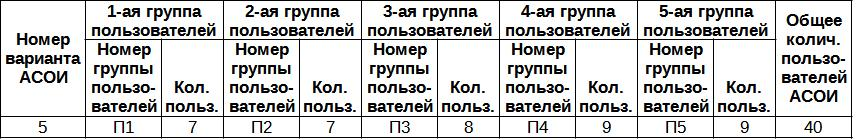
\includegraphics[width=16cm]
            {_docs/МоделиОрганизационнойСтруктурыОА.jpg}
        \caption{Модели организационной структуры ОА}
    \end{figure}

    \begin{figure}[h!]
        \centering
        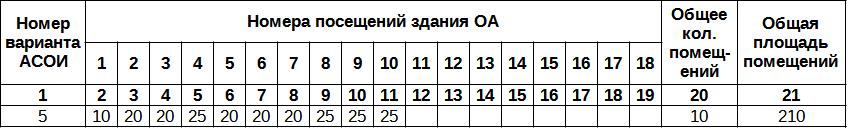
\includegraphics[width=16cm]
            {_docs/КаталогПомещенийЗданияИИхПлощадь.jpg}
        \caption{Каталог помещений здания и их площадь}
    \end{figure}

    \begin{figure}[h!]
        \centering
        % \includegraphics[]
            % {_docs/ВариантыОбщейМоделиФункциональнойСтруктурыОА.jpg}
        \caption{Варианты общей модели функциональной структуры ОА}
    \end{figure}

    \begin{figure}[h!]
        \centering
        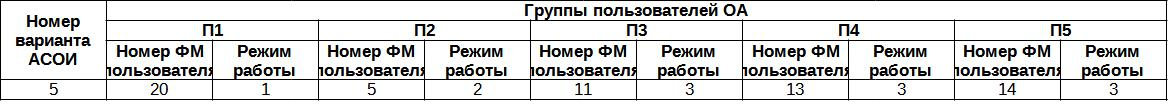
\includegraphics[width=16cm]
            {_docs/ВариантыРежимовРаботыГруппПользователейОА.jpg}
        \caption{Варианты режимов работы групп пользователей ОА}
    \end{figure}

    \begin{figure}[h!]
        \centering
        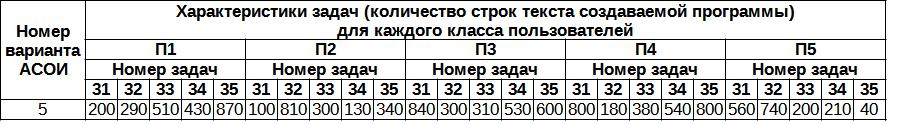
\includegraphics[width=16cm]
            {_docs/КаталогХарактеристикЗадачГруппПользователей.jpg}
        \caption{Каталог характеристик задач групп пользователей}
    \end{figure}

    \begin{figure}[ph!]
        \centering
        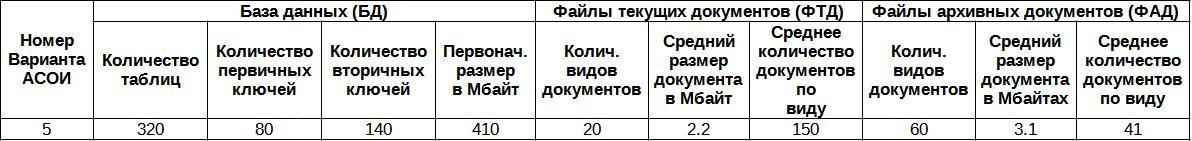
\includegraphics[width=16cm]
            {_docs/КаталогЭлементовИнформационнойСтруктурыОА.jpg}
        \caption{Каталог элементов информационной структуры ОА}
    \end{figure}

    \begin{figure}[ph!]
        \centering
        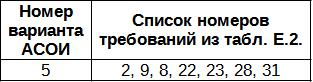
\includegraphics[]
            {_docs/ПереченьТребованийКСистемнымИИнструментальнымПрограммам.jpg}
        \caption{Перечень требований к системным и инструментальным программам}
    \end{figure}

    \begin{figure}[ph!]
        \centering
        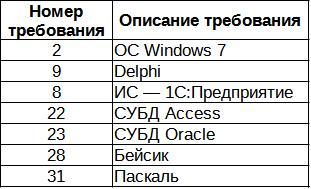
\includegraphics[]
            {_docs/КаталогТребованийКСистемнымИИнструментальнымПрограммам.jpg}
        \caption{Каталог требований к системным и инструментальным программам}
    \end{figure}

    \begin{figure}[ph!]
        \centering
        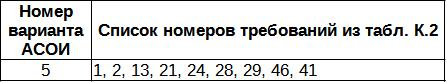
\includegraphics[]
            {_docs/ПереченьНомеровТребованийКТехническимСредствамАСОИ.jpg}
        \caption{Перечень номеров требований к техническим средствам АСОИ}
    \end{figure}

    \begin{figure}[ph!]
        \centering
        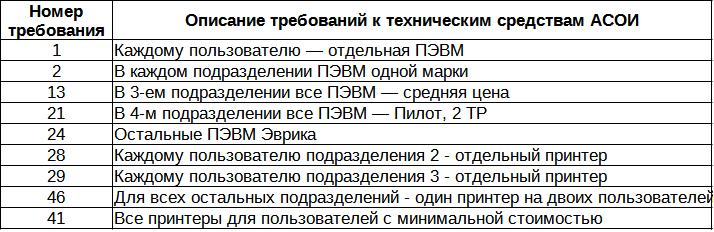
\includegraphics[]
            {_docs/КаталогТребованийКТехническимСредствамАСОИ.jpg}
        \caption{Каталог требований к техническим средствам АСОИ}
    \end{figure}

    \begin{figure}[ph!]
        \centering
        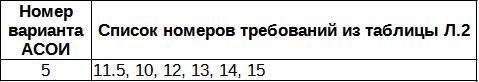
\includegraphics[]
            {_docs/СпискиНомеровТребованийКПроцессамЖЦАСОИ.jpg}
        \caption{Списки номеров требований к процессам ЖЦ АСОИ}
    \end{figure}

    \begin{figure}[ph!]
        \centering
        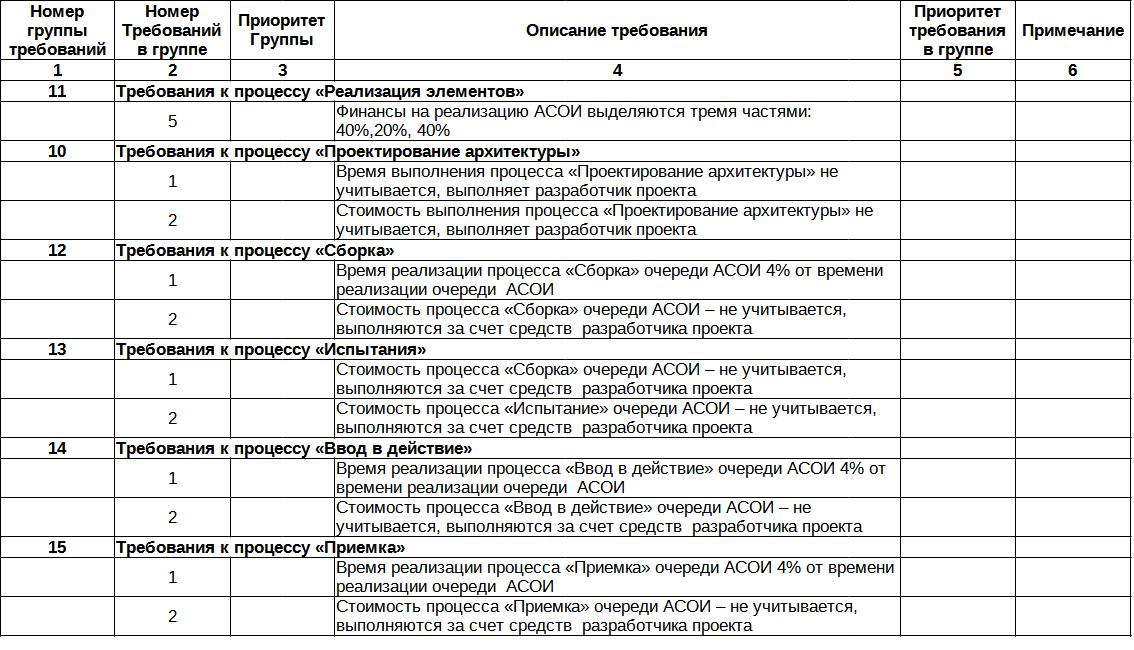
\includegraphics[width=16cm]
            {_docs/КаталогТребованийКПроцессамЖЦАСОИ.jpg}
        \caption{Каталог требований к процессам ЖЦ АСОИ}
    \end{figure}

    \begin{figure}[ph!]
        \centering
        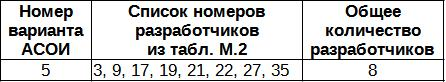
\includegraphics[]
            {_docs/СпискиНомеровРазработчиковЭлементовАСОИ.jpg}
        \caption{Списки номеров разработчиков элементов АСОИ}
    \end{figure}

    \begin{figure}[ph!]
        \centering
        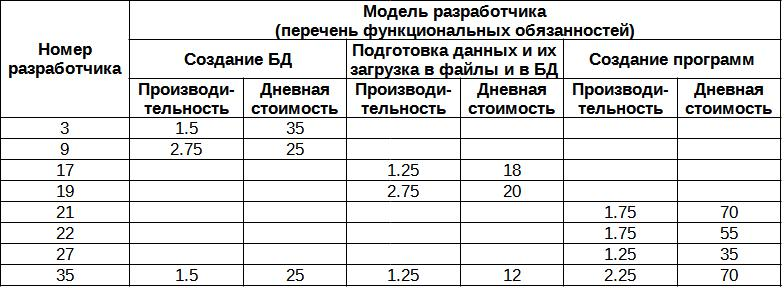
\includegraphics[]
            {_docs/КаталогРазработчиковЭлементовАСОИ.jpg}
        \caption{Каталог разработчиков элементов АСОИ}
    \end{figure}

    \newpage

    ...

%     \paragraph{} \textbf{Исходный код}: 

%     \lstinputlisting[language=c]{src/HelloWorld.c}

%     \begin{lstlisting}[caption=Вывод в консоль]
%  Hello, World!
% \end{lstlisting}

%     \paragraph{} \textbf{Вывод}: создали отчёт, используя \LaTeX.

    % % = = = = = = = =
    % % \newpage
    % % \addcontentsline{toc}{section}{Список использованных источников}
    % \section*{Список использованных источников}
    % \begin{enumerate}
    %     \item[1.] eskdx.pdf [Электронный ресурс]
    %     - Режим доступа: \url{http://tug.ctan.org/macros/latex/contrib/eskdx/manual/eskdx.pdf}.
    %     Дата~доступа:~20.02.2022.
    %     \item[2.] Опции пакета hyperref [Электронный ресурс]
    %     - Режим доступа: \url{https://grammarware.net/text/syutkin/hyperref_options.pdf}.
    %     Дата~доступа:~20.02.2022.
    % \end{enumerate}
    % \newpage
\end{document}
